% !TEX root=report.tex
\subsection{Competitor Sets} \label{subsec:competitor_sets}

The data we received from CouchSurfing does not allow us to know exactly when a host has looked at a couch request, but it does have timestamps for every request and every decision made by a host.
To form sets of ``competing'' requests, we use a heuristic procedure to scan through all requests made to a particular host, and split them into groups based on their timing, their requested lodging dates, and the timing of the host's decisions.

In the following, requests carry the same index as the user/surfer that invoked them, i.e., surfer $s_i$ sends request $c_{i,j}$ to host $h_j$.
Without loss of generality we can assume for now that each user just sends at most one request to each couch.
In the following examples, $h$ is fixed, so we just denote requests as $c_i$.
 
The CS system allows hosts to reject a couch request, which indicates a negative sample. We call those \textit{explicit negatives}. In addition, it is possible to infer \textit{implicit negatives}: if we take for example a host $h$ with a very popular couch in Paris with tens of requests per day, it seems reasonable to assume that $h$ will not look at every request, and will stop reading more requests after deciding for a specific surfer $s_i$.
These requests won't receive an explicit Reject, but are \emph{de facto} rejected due to ``timing out.''

For a given period $\tau$, let $C_{j}^{\tau} = c_1, c_2,\ldots,c_n$ be the requests send to $h$. We hereby assume that if at a certain time host $h$ accepts a request $c_i$ for period $\tau$, she prefers the requesting surfer $s_i$ over all other users whose requests she read that overlap with $\tau$. An efficient sweep-line algorithm to find sets of overlapping requests is depicted in {algorithm~\ref{alg:overlap}}.

One more important thing to keep in mind is that if $h$ accepted a request for period $\tau$ at time $t_0$ and gets another request $c_l$ for $\tau$ at time $t_1 > t_0$, there is no information about whether or not $h$ likes $s_i$, because his couch is already taken, so we have to filter these out before moving on.

\begin{algorithm}
\caption{Find overlapping requests}
\label{alg:overlap}
\begin{algorithmic} 
\REQUIRE $R = (c_1, c_2,\ldots,c_n)$, $c_i = (t_i^{start}, t_i^{end})$
\ENSURE $S\subseteq \mathcal{P}(R)$ 
\STATE $S \leftarrow \emptyset$
\STATE $A \leftarrow \emptyset$ 
\STATE $T {(i, start/end, t_i^{s/t}) |c_i \in R}$
\STATE $sort(T, t_i^{s/t})$ 
\STATE $b\_incr \leftarrow True$ 
\FOR{$t$ in $T$}
\IF{$t$ == $v_j^{start}$}
\STATE $A.append(t)$
\STATE $b\_incr \leftarrow True$
\ELSE
\IF{$b\_incr == True$}
\STATE $b\_incr \leftarrow False$
\STATE $S.append({c_i | (i, \_, \_) \in A})$
\ENDIF
\STATE $A.delete(t)$
\ENDIF
\ENDFOR
\end{algorithmic}
\end{algorithm}

It might also be beneficial to soften the notion of ``overlap'' just because it might be very stressful for a host to have surfers without a gap in between the two visits.

Analyzing the data for statistics on gaps for each host seperately will reveal their willingness to host several surfers in a row.
The above algorithm can easily be adapted by modifying the input times accordingly.
\todo{for tobi: clarify this: is this used?}

\subsubsection{Filter rejects by temporal constraints}
\todo{for tobi: i'm confused---how is what was done above different from this? maybe unite?}

\todo{for tobi: insert reference to \autoref{fig:timeline_view} somewhere.}

Using a very similar technique we can filter rejects that are not actually rejects for the reason of a mismatching surfer. Imagine $h$ gets a request $c_1$ at time $t_1$, accepts this request at time $t_2$ and gets another request $c_2$ for the same period as $c_1$ at $t_3$. If we have that $t_1 < t_2 < t_3$, there is no valid information about whether or not $h$ likes surfer $s_2$. By the time he gets the second request, his couch is already booked out and so he has to reject $s_2$ no matter if he would even prefer him over $s_1$. Because of this scenario we filter our training data for exactly those \textit{uninformative rejects} using again algorithm~\ref{alg:overlap} and temporal orderings on requests and acceptances/rejects.

\begin{figure}[ht]
\centering
\subfloat[Requested]{
  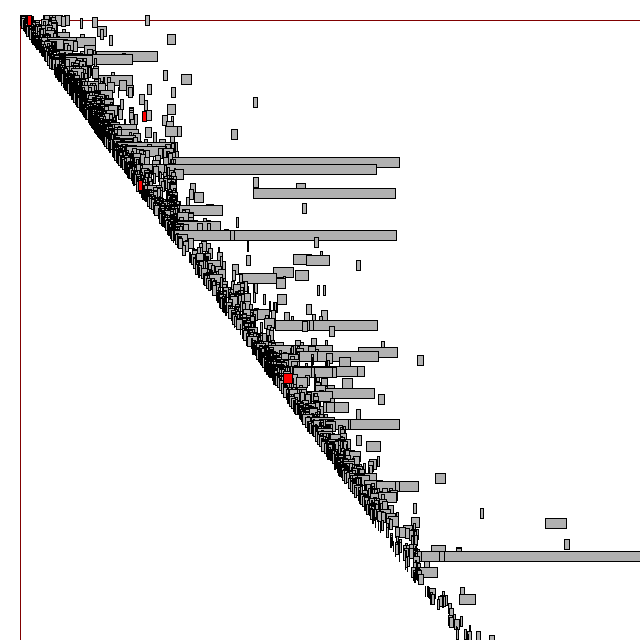
\includegraphics[width=0.45\linewidth]{figures/top_requested.png}
}
\subfloat[Accepted]{
  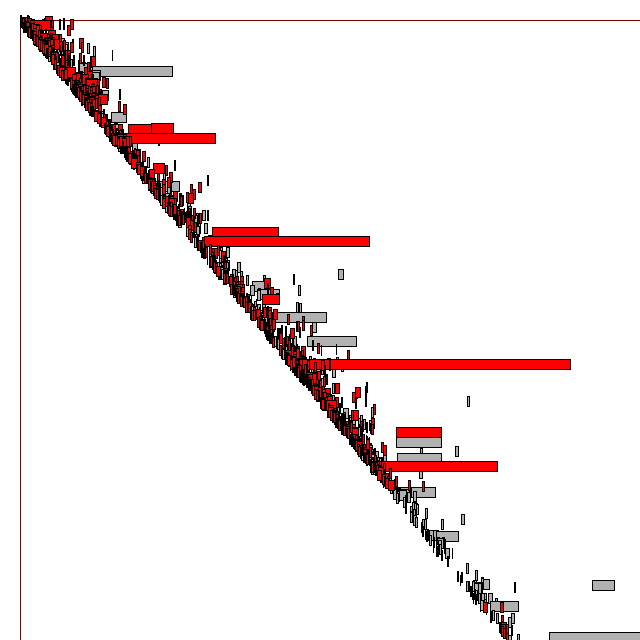
\includegraphics[width=0.45\linewidth]{figures/top_accepted.png}
}
\caption{\todo{for tobi: Explain.}}
\label{fig:timeline_view}
\end{figure}
